\section{Races}
There are ten playable races which represent the ten mainstream cultures of Tamriel. Each comes with a starting set of attributes as well as skill bonuses and special traits or powers. Each race is listed here along with a picture, description, and stats. Don't write this all in pen - it'll be changing!\\

Races begin the game with the stats listed in the following table:
\begin{figure}[h]
\begin{tabular}[h]{|p{0.1\textwidth}|p{0.1\textwidth}p{0.1\textwidth}p{0.1\textwidth}p{0.1\textwidth}p{0.1\textwidth}p{0.1\textwidth}p{0.1\textwidth}|}
	\hline
	\textbf{Race} & STR & INT & WIL & AGI & SPD & END & PER\\
	\hline
	Altmer & 30 & 50 & 40 & 40 & 35 & 35 & 40\\
	\hline
	Argonian & 40 & 45 & 35 & 45 & 45 & 30 & 30\\
	\hline
	Bosmer & 30 & 40 & 30 & 50 & 50 & 35 & 35\\
	\hline
	Breton & 35 & 50 & 50 & 30 & 35 & 30 & 40\\
	\hline
	Dunmer & 40 & 40 & 30 & 40 & 50 & 35 & 35\\
	\hline
	Imperial & 40 & 40 & 35 & 30 & 35 & 40 & 50\\
	\hline
	Khajit & 35 & 40 & 30 & 50 & 40 & 35 & 40\\
	\hline
	Nord & 50 & 30 & 35 & 40 & 40 & 45 & 30\\
	\hline
	Orc & 45 & 35 & 45 & 35 & 30 & 50 & 30\\
	\hline
	Redguard & 45 & 30 & 30 & 40 & 40 & 50 & 35\\
	\hline
\end{tabular}
\end{figure}

\subsection{Altmer (High Elf)}
\begin{wrapfigure}{L}{0.3\textwidth}
	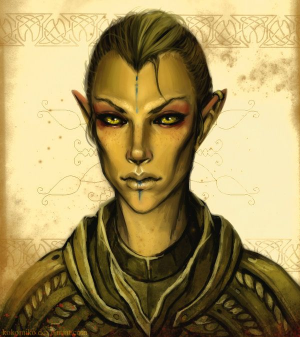
\includegraphics[width=\textwidth]{Altmer.png}
\end{wrapfigure}

The Altmer, or self-titled ``Cultured People', are a tall, golden-skinned race, hailing from Summerset Isle. They are also known as High Elves by the denizens of Tamriel. In the Empire, ``High'' is often understood to mean proud or snobbish, and as the Altmer generally personify these characteristics, the ``lesser races'' generally resent them. Altmer live two to three times as long as humans; with a 200-year-old Altmer being old and a 300-year-old Altmer being very, very old. Altmer consider themselves to be the most civilized culture of Tamriel; the common tongue of the continent is based on Altmer speech and writing, and most of the Empire's arts, crafts, laws, and sciences are derived from Altmer traditions. They usually have golden, green, or amber eyes.\\

The Altmer are the most strongly gifted in the arcane arts of all the races, and they are very resistant to diseases. However, they are also somewhat vulnerable to magicka, fire, frost, and shock, which makes them very weak against their strongest point --- magic. They are among the longest living and most intelligent races of Tamriel, and they often become powerful magic users due to both their magical affinity and the many years they may devote to their studies.\\

Altmer get the following skill bonuses: +5 Alchemy, +10 Alteration, +5 Conjuration, +10 Destruction, +5 Illusion, +10 Mysticism.\\

Altmer have a permanent +100 bonus to max magicka and a 75\% resistance to disease; however, they have a 25\% vulnerability to fire, frost and shock damage.

\subsection{Argonian}
\begin{wrapfigure}{L}{0.3\textwidth}
	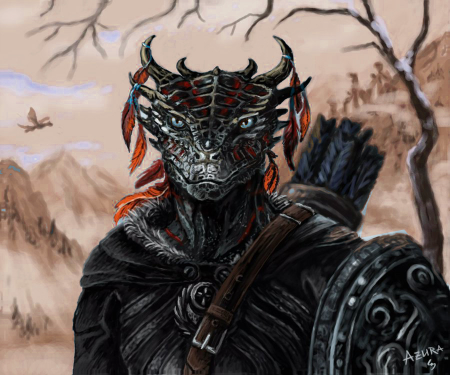
\includegraphics[width=\textwidth]{Argonian.png}
\end{wrapfigure}

Argonians (in their native tongue of Jel they call themselves the Saxhleel, or People of the Root) are the reptilian natives of Black Marsh, a vast swampland province in southeastern Tamriel. The other races often prefer to refer to them as 'lizards' or the 'Lizard Folk' instead, especially when meaning to be derogative. They are known as the foremost experts in guerrilla warfare throughout the Starry Heart, a reputation brought upon them by defending their borders from enemies for countless centuries. Argonians have a lifespan similar to that of humans. According to the First Era Scholar Brendan the Persistent "the Argonian people have, throughout Tamrielic history, been perhaps the most misunderstood, vilified, and reviled of all the sentient races. Yet, those who have taken the time to experience Argonian culture have gained a greater appreciation for this noble and beautiful people." However, it should be noted that he himself went missing in his final expedition into the deeper swamps of their homeland.\\

Argonians get the following skill bonuses: +5 Alchemy, +10 Athletics, +5 Blade, +5 Hand-to-Hand, +5 Illusion, +5 Mysticism, +10 Security.\\

They have a complete immunity to poison and a 75\% resistance to disease. They can breathe underwater and are adept swimmers, suffering no movement penalty or melee attack penalty in water.

\subsection{Bosmer (Wood Elf)}
\begin{wrapfigure}{L}{0.3\textwidth}
	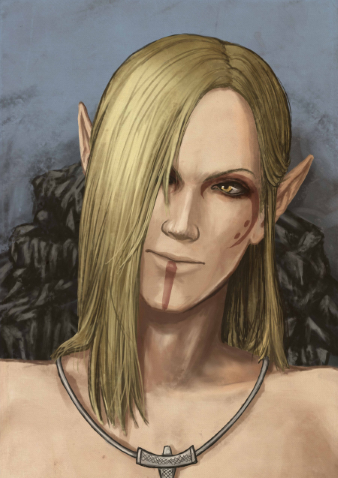
\includegraphics[width=\textwidth]{Bosmer.png}
\end{wrapfigure}

The Bosmer are the Elven clan-folk of Valenwood, a forested province in southwestern Tamriel. In the Empire, they are often referred to as Wood Elves, but Bosmer, Boiche, or the Tree-Sap people is what they call themselves. Bosmer rejected the stiff, formal traditions of Aldmeri high culture, preferring a more romantic, simple existence in harmony with the land and its wild beauty and creatures. They are relatively nimble and quick in body compared to their more "civilized" Altmeri cousins (who often look down upon the Bosmer as unruly and naive). Their agility makes them well-suited as scouts and thieves. However, they are also a quick-witted folk, and many pursue successful careers in scholarly pursuits or trading. Bosmer live two to three times as long as humans; with a 200-year-old Bosmer being old and a 300-year-old Bosmer being very, very old. Though they are considered less influential than some of their Elven brethren, the Bosmer are also relatively prone to producing offspring. As a result, they outnumber all other mer on Tamriel.\\

The best archers in all of Tamriel, the Bosmer snatch and fire arrows in one continuous motion; they are even rumored to have invented the bow. They have many natural and unique abilities; notably, they can command simple-minded creatures and have a nearly chameleon-like ability to hide in forested areas. Many in the forests of Valenwood follow the tenets of the Green Pact. These "Green Pact Bosmer" are religiously carnivorous and cannibalistic, and do not harm the vegetation of Valenwood, though they are not averse to using wooden or plant-derived products created by others.\\

Bosmer get the following skill bonuses: +5 Acrobatics, +10 Alchemy, +5 Alteration, +5 Light Armor, +10 Marksman, +10 Sneak.\\

Bosmer have a 75\% resistance to disease. They get the Beast Tongue power as well, which lets them control lesser animals for 1 minute once a day.

\subsection{Breton}
\begin{wrapfigure}{L}{0.3\textwidth}
	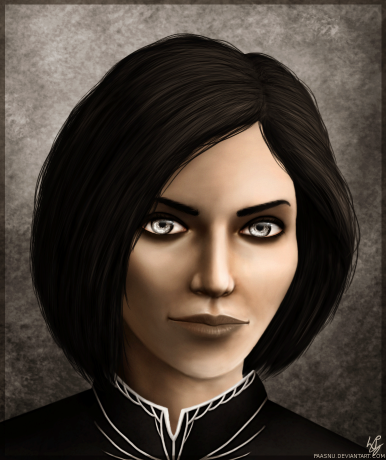
\includegraphics[width=\textwidth]{Breton.png}
\end{wrapfigure}

Bretons are the human descendants of the Aldmeri-Nedic Manmer of the Merethic Era and are now the inhabitants of the province of High Rock. They are united in culture and language, even though they are divided politically, for High Rock is a fractious region. Bretons make up the peasantry, soldiery, and magical elite of the feudal kingdoms that compete for power. Many are capable mages with innate resistance to magicka. They are known for a proficiency in abstract thinking and unique customs. Bretons appear, by and large, much like other pale-skinned humans. They are usually slight of build and not as muscular as Nords or Redguards. Their Elvish ancestry is usually only detectable upon a closer inspection of their eyebrows, ears, or high cheekbones, though many individual Bretons appear to be more Nordic or Imperial than anything else. The great diversity in their appearance is to be expected from their politically fractured society, though their clothes, accents, customs and names are fairly uniform.\\

Bretons get the following skill bonuses: +5 Alchemy, +5 Alteration, +10 Conjuration, +5 Illusion, +10 Mysticism, +10 Restoration.\\

They have a natural 50\% resistance to magic and gain a permanent +50 bonus to max magicka. Their Dragon Skin power gives them 50\% physical resistance for 1 minute, once a day.

\subsection{Dunmer (Dark Elf)}
\begin{wrapfigure}{L}{0.3\textwidth}
	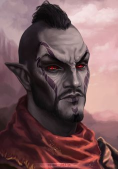
\includegraphics[width=\textwidth]{Dunmer.png}
\end{wrapfigure}

The Dunmer, also known as Dark Elves, are the ash-skinned, typically red-eyed elven peoples of Morrowind. ``Dark'' is commonly understood as meaning such characteristics as ``dark-skinned'', ``gloomy'', ``ill-favored by fate'' and so on. The Dunmer and their national identity, however, embrace these various connotations with enthusiasm. In the Empire, ``Dark Elf'' is the common usage, but among their Aldmeri brethren they are called ``Dunmer''. Their combination of powerful intellects with strong and agile physiques produce superior warriors and sorcerers. On the battlefield, Dunmer are noted for their skill with a balanced integration of the sword, the bow and destruction magic. Dunmer live two to three times as long as humans; with a 200-year-old Dunmer being old and a 300-year-old Dunmer being very, very old. In character, they are grim, aloof, and reserved, as well as distrusting and disdainful of other races.\\

Dunmer distrust and are treated distrustfully by other races. They are often proud, clannish, ruthless, and cruel, from an outsider's point of view, but greatly value loyalty and family. Young female Dunmer have a reputation for promiscuity in some circles. Despite their powerful skills and strengths, the Dunmer's vengeful nature, age-old conflicts, betrayals, and ill-reputation prevent them from gaining more influence. Those born in their homeland of Morrowind are known to be considerably less friendly than those who grew up in the Imperial tradition.\\

Dunmer get the following skill bonuses: +5 Athletics, +10 Blade, +5 Blunt, +10 Destruction, +5 Light Armor, +5 Marksman, +5 Mysticism.\\

Dunmer have a natural 75\% resistance to fire. They can also summon an ancestral spirit to aid them in battle for 1 minute, once a day.

\newpage % Gets the float to align properly
\subsection{Imperial}
\begin{wrapfigure}{l}{0.3\textwidth}
	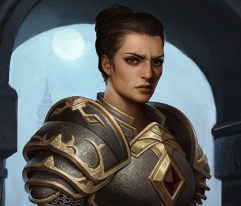
\includegraphics[width=\textwidth]{Imperial.png}
\end{wrapfigure}

Also known as Cyrodiils, Cyrodilics, Cyro-Nordics and Imperial Cyrods, the well-educated and well-spoken Imperials are the natives of the civilized, cosmopolitan province of Cyrodiil. Imperials are also known for the discipline and training of their citizen armies, and their respect for the rule of law. Though physically less imposing than the other races, the Imperials have proved to be shrewd diplomats and traders, and these traits, along with their remarkable skill and training as light infantry, have enabled them to subdue all the other nations and races and erect the monument to peace and prosperity that comprises the Glorious Empire. Their hegemony has waxed and waned throughout the eras, and most historians refer to three distinct Empires, the ends of which each mark a new epoch in Tamrielic history.\\

Imperials get the following skill bonuses: +5 Blade, +5 Blunt, +5 Hand-to-Hand, +10 Heavy Armor, +10 Mercantile, +10 Speechcraft.\\

Imperials gain two major powers: Star of the West, which lets them absorb 100 stamina on touch once per day, and Voice of the Emperor, which charms a target for 30 seconds once per day.

\subsection{Khajiit}
\begin{wrapfigure}{l}{0.3\textwidth}
	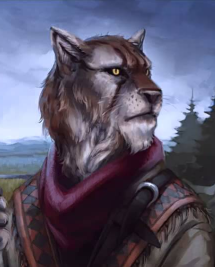
\includegraphics[width=\textwidth]{Khajiit.png}
\end{wrapfigure}

Khajiit are cat-like people who come from Elsweyr, known for high intelligence and agility. These traits make them very good thieves and acrobats, but Khajiit are also fearsome warriors. However, they are rarely known to be mages. Khajiit mostly stay on land, but piracy and skooma trade does draw some to work as sailors.\\

Khajiit anatomy differs greatly from both men and elves, not only because of their fur, tail, and sometimes toe-walking stance, but also their digestive system and metabolism. Khajiit, Argonians, and Imga are the so-called ``beast races'' of Tamriel because of these large differences. Khajiit have a lifespan similar to that of humans. There are no well-documented cases of cross-breeding between Khajiit and other races, though there are rumors of such a thing. The foreign appearance and behavior of Khajiit make them common targets of racial discrimination.\\

Khajiit get the following skill bonuses: +10 Acrobatics, +5 Athletics, +5 Blade, +10 Hand-to-Hand, +5 Light Armor, +5 Security, +5 Sneak.\\

Khajiit have cat eyes that allow them to see in the dark and claws that boost their unarmed attack damage to 1d6+DB. In addition to this, the Eye of Fear power lets them inflict fear for 3 rounds on a single target who can see them, once a day.

\subsection{Nord}
\begin{wrapfigure}{l}{0.3\textwidth}
	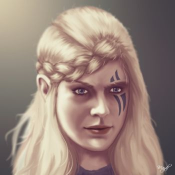
\includegraphics[width=\textwidth]{Nord.png}
\end{wrapfigure}

The Nords are the children of the sky, a race of tall and fair-haired humans from Skyrim who are known for their incredible resistance to cold and magical frost. They are fierce, strong and enthusiastic warriors, and many become renowned warriors, soldiers and mercenaries all over Tamriel. Eager to augment their martial skills beyond the traditional methods of Skyrim, they excel in all manner of warfare, and are known as a militant people by their neighbors. Nords are also natural seamen, and have benefited from nautical trade since their first migrations from Atmora. They captain and crew many merchant fleets, and may be found all along the coasts of Tamriel.\\

Nords get the following skill bonuses: +5 Armorer, +10 Blade, +5 Block, +10 Blunt, +10 Heavy Armor, +5 Restoration.\\

Nords have a 50\% resistance to frost damage and can channel Nordic Frost to deal 50 points of frost damage on touch once per day. The Woad power grants them 30\% physical damage reduction for one minute once per day.

\subsection{Orc}
\begin{wrapfigure}{l}{0.3\textwidth}
	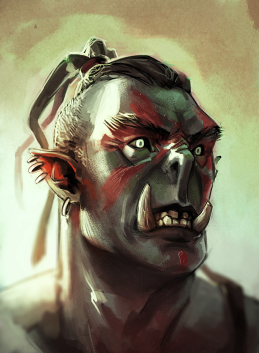
\includegraphics[width=\textwidth]{Orc.png}
\end{wrapfigure}

Orcs, also called Orsimer or "Pariah Folk" in ancient times, are sophisticated, beastlike people of the Wrothgarian Mountains, Dragontail Mountains, Valenwood, and Orsinium (literally translated as ``Orc-Town''). They are noted for their unshakable courage in war and their unflinching endurance of hardships. Orcs have elven blood, but are usually considered to be beastfolk. In the past, Orcs have been widely feared and hated by the other nations and races of Tamriel, and were often considered to be goblin-ken. However, they have slowly won acceptance in the Empire, in particular for their distinguished service in the Emperor's Legions. Orc armorers are prized for their craftsmanship, and Orc warriors in heavy armor are among the finest front-line troops in the Empire, and are fearsome when using their berserker rage. Orcs have a lifespan similar to that of humans. Most Imperial citizens regard the Orc society as rough and cruel. The Orcs of the Iliac Bay region have developed their own language, known as Orcish, and have often had their own kingdom, Orsinium.\\

Orcs get the following skill bonuses: +10 Armorer, +5 Block, +10 Blunt, +5 Hand-to-Hand, +10 Heavy Armor.\\

Orcs have a natural 25\% resistance to magic. Once a day they may enter a berserk state for 1 minute, which grants the following effects: Fortify Stamina 200, Fortify Health 20, Fortify Strength 50, Drain Agility 100.

\subsection{Redguard}
\begin{wrapfigure}{l}{0.3\textwidth}
	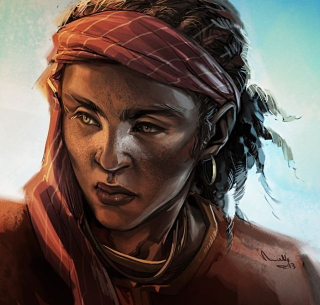
\includegraphics[width=\textwidth]{Redguard.png}
\end{wrapfigure}

Redguards are the most naturally talented warriors in Tamriel. The dark-skinned, wiry-haired people of Hammerfell seem born to battle, though their pride and fierce independence of spirit makes them more suitable as scouts or skirmishers, or as free-ranging heroes and adventurers, than as rank-and-file soldiers. In addition to their cultural affinities for many armor styles and weapons (particularly swords), Redguards are also physically blessed with hardy constitutions, resistance to poison, and quickness of foot. Redguards do not share the same blood as the other human races, and they have no known connection with the ancestral Nordic homeland of Atmora.\\

Redguards get the following skill bonuses: +10 Athletics, +10 Blade, +10 Blunt, +5 Heavy Armor, +5 Light Armor, +5 Mercantile.\\

Hardy of constitution, Redguards have a natural 75\% resistance to poison and disease. Once a day, they can have an Adrenaline Rush which grants the following effects for 1 minute: Fortify Agility 50, Fortify Endurance 50, Fortify Speed 50, Fortify Strength 50, Fortify Health 25.\\

\begin{tcolorbox}
Be sure to take note of all your race's skill bonuses and abilities. Skills will be covered in greater detail in the next chapter, so you may wish to come back here once you learn more about them.
\end{tcolorbox}